% Created by tikzDevice version 0.8.1 on 2015-06-10 21:23:14
% !TEX encoding = UTF-8 Unicode
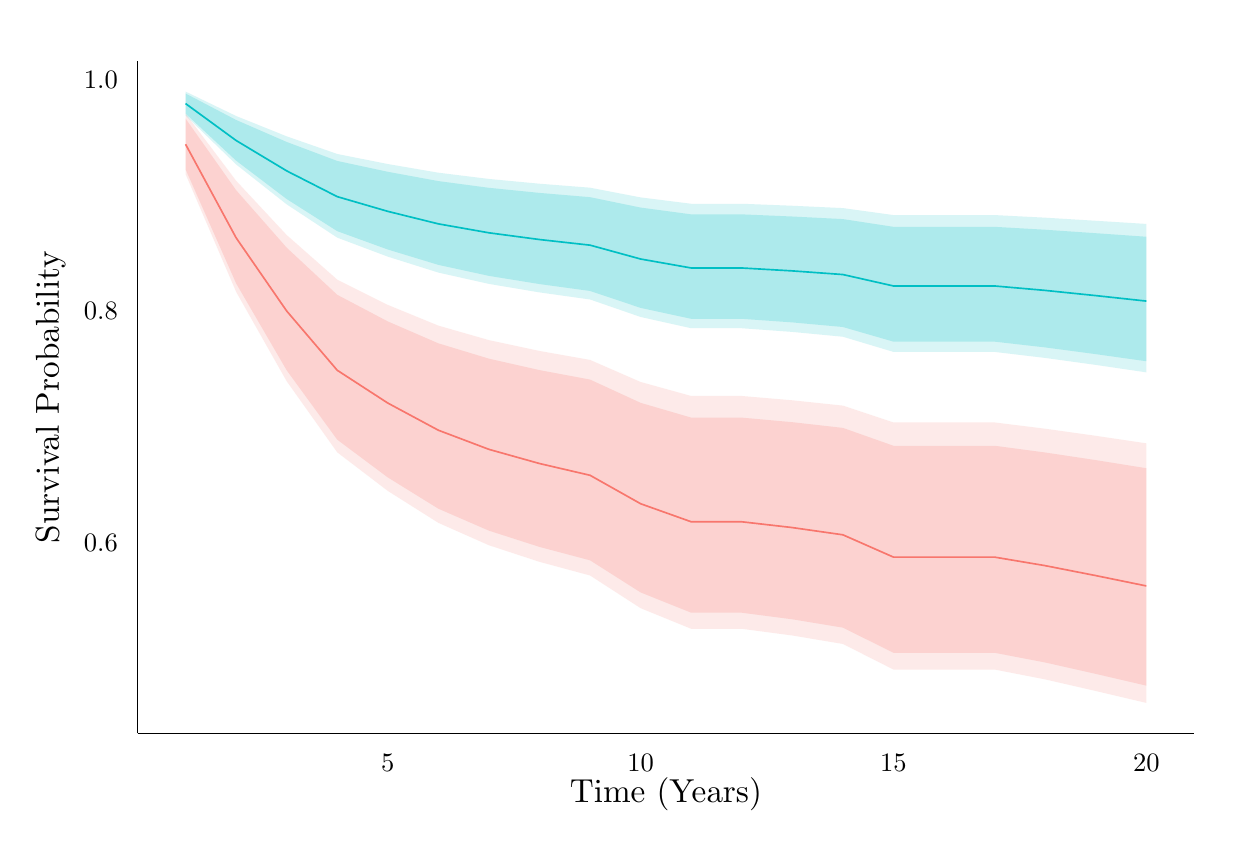
\begin{tikzpicture}[x=1pt,y=1pt]
\definecolor{fillColor}{RGB}{255,255,255}
\path[use as bounding box,fill=fillColor,fill opacity=0.00] (0,0) rectangle (433.62,289.08);
\begin{scope}
\path[clip] (  0.00,  0.00) rectangle (433.62,289.08);
\definecolor{drawColor}{RGB}{255,255,255}
\definecolor{fillColor}{RGB}{255,255,255}

\path[draw=drawColor,line width= 0.6pt,line join=round,line cap=round,fill=fillColor] (  0.00,  0.00) rectangle (433.62,289.08);
\end{scope}
\begin{scope}
\path[clip] ( 39.69, 34.03) rectangle (421.57,277.03);
\definecolor{fillColor}{RGB}{255,255,255}

\path[fill=fillColor] ( 39.69, 34.03) rectangle (421.58,277.03);
\definecolor{drawColor}{RGB}{248,118,109}

\path[draw=drawColor,line width= 0.6pt,line join=round] ( 57.05,246.95) --
	( 75.32,213.14) --
	( 93.59,186.70) --
	(111.86,165.28) --
	(130.13,153.43) --
	(148.41,143.61) --
	(166.68,136.70) --
	(184.95,131.58) --
	(203.22,127.33) --
	(221.49,117.05) --
	(239.77,110.53) --
	(258.04,110.53) --
	(276.31,108.44) --
	(294.58,105.82) --
	(312.86, 97.76) --
	(331.13, 97.76) --
	(349.40, 97.76) --
	(367.67, 94.68) --
	(385.94, 91.09) --
	(404.22, 87.35);
\definecolor{drawColor}{RGB}{0,191,196}

\path[draw=drawColor,line width= 0.6pt,line join=round] ( 57.05,261.65) --
	( 75.32,248.31) --
	( 93.59,237.33) --
	(111.86,228.02) --
	(130.13,222.70) --
	(148.41,218.18) --
	(166.68,214.95) --
	(184.95,212.52) --
	(203.22,210.49) --
	(221.49,205.48) --
	(239.77,202.24) --
	(258.04,202.24) --
	(276.31,201.19) --
	(294.58,199.87) --
	(312.86,195.74) --
	(331.13,195.74) --
	(349.40,195.74) --
	(367.67,194.14) --
	(385.94,192.26) --
	(404.22,190.28);
\definecolor{fillColor}{RGB}{248,118,109}

\path[fill=fillColor,fill opacity=0.15] ( 57.05,258.02) --
	( 75.32,233.76) --
	( 93.59,214.15) --
	(111.86,198.03) --
	(130.13,188.90) --
	(148.41,181.41) --
	(166.68,176.17) --
	(184.95,172.26) --
	(203.22,169.02) --
	(221.49,161.05) --
	(239.77,155.99) --
	(258.04,155.99) --
	(276.31,154.43) --
	(294.58,152.51) --
	(312.86,146.43) --
	(331.13,146.43) --
	(349.40,146.43) --
	(367.67,144.16) --
	(385.94,141.60) --
	(404.22,138.88) --
	(404.22, 45.08) --
	(385.94, 49.39) --
	(367.67, 53.58) --
	(349.40, 57.14) --
	(331.13, 57.14) --
	(312.86, 57.14) --
	(294.58, 66.38) --
	(276.31, 69.44) --
	(258.04, 71.86) --
	(239.77, 71.86) --
	(221.49, 79.31) --
	(203.22, 91.12) --
	(184.95, 96.06) --
	(166.68,102.05) --
	(148.41,110.14) --
	(130.13,121.69) --
	(111.86,135.63) --
	( 93.59,161.33) --
	( 75.32,193.63) --
	( 57.05,236.18) --
	cycle;
\definecolor{fillColor}{RGB}{0,191,196}

\path[fill=fillColor,fill opacity=0.15] ( 57.05,265.99) --
	( 75.32,257.16) --
	( 93.59,249.81) --
	(111.86,243.44) --
	(130.13,239.80) --
	(148.41,236.67) --
	(166.68,234.41) --
	(184.95,232.69) --
	(203.22,231.25) --
	(221.49,227.74) --
	(239.77,225.45) --
	(258.04,225.45) --
	(276.31,224.73) --
	(294.58,223.88) --
	(312.86,221.36) --
	(331.13,221.36) --
	(349.40,221.36) --
	(367.67,220.42) --
	(385.94,219.30) --
	(404.22,218.16) --
	(404.22,164.53) --
	(385.94,167.22) --
	(367.67,169.74) --
	(349.40,171.91) --
	(331.13,171.91) --
	(312.86,171.91) --
	(294.58,177.40) --
	(276.31,179.14) --
	(258.04,180.47) --
	(239.77,180.47) --
	(221.49,184.54) --
	(203.22,190.86) --
	(184.95,193.42) --
	(166.68,196.49) --
	(148.41,200.58) --
	(130.13,206.34) --
	(111.86,213.21) --
	( 93.59,225.24) --
	( 75.32,239.66) --
	( 57.05,257.35) --
	cycle;
\definecolor{fillColor}{RGB}{248,118,109}

\path[fill=fillColor,fill opacity=0.20] ( 57.05,256.22) --
	( 75.32,230.36) --
	( 93.59,209.59) --
	(111.86,192.55) --
	(130.13,182.93) --
	(148.41,175.01) --
	(166.68,169.47) --
	(184.95,165.34) --
	(203.22,161.92) --
	(221.49,153.51) --
	(239.77,148.17) --
	(258.04,148.17) --
	(276.31,146.52) --
	(294.58,144.46) --
	(312.86,138.00) --
	(331.13,138.00) --
	(349.40,138.00) --
	(367.67,135.57) --
	(385.94,132.82) --
	(404.22,129.89) --
	(404.22, 51.32) --
	(385.94, 55.57) --
	(367.67, 59.69) --
	(349.40, 63.19) --
	(331.13, 63.19) --
	(312.86, 63.19) --
	(294.58, 72.28) --
	(276.31, 75.29) --
	(258.04, 77.67) --
	(239.77, 77.67) --
	(221.49, 85.00) --
	(203.22, 96.60) --
	(184.95,101.45) --
	(166.68,107.32) --
	(148.41,115.25) --
	(130.13,126.56) --
	(111.86,140.20) --
	( 93.59,165.28) --
	( 75.32,196.69) --
	( 57.05,237.89) --
	cycle;
\definecolor{fillColor}{RGB}{0,191,196}

\path[fill=fillColor,fill opacity=0.20] ( 57.05,265.29) --
	( 75.32,255.73) --
	( 93.59,247.78) --
	(111.86,240.92) --
	(130.13,237.00) --
	(148.41,233.64) --
	(166.68,231.21) --
	(184.95,229.37) --
	(203.22,227.83) --
	(221.49,224.07) --
	(239.77,221.62) --
	(258.04,221.62) --
	(276.31,220.84) --
	(294.58,219.91) --
	(312.86,217.11) --
	(331.13,217.11) --
	(349.40,217.11) --
	(367.67,216.06) --
	(385.94,214.81) --
	(404.22,213.53) --
	(404.22,168.54) --
	(385.94,171.11) --
	(367.67,173.54) --
	(349.40,175.62) --
	(331.13,175.62) --
	(312.86,175.62) --
	(294.58,180.91) --
	(276.31,182.58) --
	(258.04,183.87) --
	(239.77,183.87) --
	(221.49,187.82) --
	(203.22,193.94) --
	(184.95,196.43) --
	(166.68,199.39) --
	(148.41,203.36) --
	(130.13,208.92) --
	(111.86,215.55) --
	( 93.59,227.16) --
	( 75.32,241.03) --
	( 57.05,258.04) --
	cycle;
\end{scope}
\begin{scope}
\path[clip] (  0.00,  0.00) rectangle (433.62,289.08);
\definecolor{drawColor}{RGB}{0,0,0}

\path[draw=drawColor,line width= 0.6pt,line join=round] ( 39.69, 34.03) --
	( 39.69,277.03);
\end{scope}
\begin{scope}
\path[clip] (  0.00,  0.00) rectangle (433.62,289.08);
\definecolor{drawColor}{RGB}{0,0,0}

\node[text=drawColor,anchor=base east,inner sep=0pt, outer sep=0pt, scale=  0.96] at ( 32.57, 99.82) {0.6};

\node[text=drawColor,anchor=base east,inner sep=0pt, outer sep=0pt, scale=  0.96] at ( 32.57,183.52) {0.8};

\node[text=drawColor,anchor=base east,inner sep=0pt, outer sep=0pt, scale=  0.96] at ( 32.57,267.22) {1.0};
\end{scope}
\begin{scope}
\path[clip] (  0.00,  0.00) rectangle (433.62,289.08);
\definecolor{drawColor}{RGB}{0,0,0}

\path[draw=drawColor,line width= 0.6pt,line join=round] ( 39.69, 34.03) --
	(421.57, 34.03);
\end{scope}
\begin{scope}
\path[clip] (  0.00,  0.00) rectangle (433.62,289.08);
\definecolor{drawColor}{RGB}{0,0,0}

\node[text=drawColor,anchor=base,inner sep=0pt, outer sep=0pt, scale=  0.96] at (130.13, 20.31) {5};

\node[text=drawColor,anchor=base,inner sep=0pt, outer sep=0pt, scale=  0.96] at (221.49, 20.31) {10};

\node[text=drawColor,anchor=base,inner sep=0pt, outer sep=0pt, scale=  0.96] at (312.86, 20.31) {15};

\node[text=drawColor,anchor=base,inner sep=0pt, outer sep=0pt, scale=  0.96] at (404.22, 20.31) {20};
\end{scope}
\begin{scope}
\path[clip] (  0.00,  0.00) rectangle (433.62,289.08);
\definecolor{drawColor}{RGB}{0,0,0}

\node[text=drawColor,anchor=base,inner sep=0pt, outer sep=0pt, scale=  1.20] at (230.63,  9.03) {Time (Years)};
\end{scope}
\begin{scope}
\path[clip] (  0.00,  0.00) rectangle (433.62,289.08);
\definecolor{drawColor}{RGB}{0,0,0}

\node[text=drawColor,rotate= 90.00,anchor=base,inner sep=0pt, outer sep=0pt, scale=  1.20] at ( 11.28,155.53) {Survival Probability};
\end{scope}
\end{tikzpicture}
